\documentclass[12pt]{base}

\definecolor{LightCyan}{rgb}{0.88,1,1}

\date{ }

\begin{document}

\begin{titlepage}

\begin{center}
    \vspace*{5cm}
    \huge ARCHITECTURE - TP05\\
    \text{ }\\
    \LARGE L2 Informatique\\
    \vfill
    \LARGE WAHARTE Mathieu\\
\end{center}

\end{titlepage}

\newpage

\section{Produit scalaire}

% Brouillon

% politique LRU\newline
% échec de capacité, conflit, démarage
% pk impact associativité ?\newline

% N donne la taille de des tableaux X et Y $\Ra$ des "blocs" à prendre pour pouvoir les lire\\
% Pour N = 64 \ref{fig:1_64}, quand la taille de la ligne est de 16, il y a 50\% de chance de tomber sur un échec de capacité puisque l'on ne peut pas faire tenir les blocs de donnée contenant tout X (resp. Y) dans ceux du cache (ceci est donc indépendant du niveau d'associativité ou du nombre de blocs comme remarqué). On a bien aucun échec de conflit car on n'observe aucune variation de du nombre d'erreurs avec le niveau d'associativité.
% \newline

% N=64, bloc = 16 $\ra$ 256 blocs, à chaque cycle on fait x[i]*y[i] donc cache charge x = 64 dans les 4 premiers blocs et y = 64 dans les 4 suivants par ex. Il doit aussi stocker la somme partielle s, qui prends 64 bits donc prends les 4 suivantes.






\begin{figure}[H]
\centering
\begin{tikzpicture}
\draw[red, thick] (0,0) rectangle (10,10);
\node[red] at (5,10.3){total cache size};
%-- version with the label on the side --
%\node[left,red] at (-2,5){total cache size};
%\draw[->, red] (-3,5.2) .. controls (-2.3,9.3) .. (-0.1,9.8);

\node[left,blue] at (-0.7,8){set};
\draw[blue] (0,8.4) -- (10,8.4);
\draw[blue] (0,7.4) -- (10, 7.4);
%\draw[blue] (0,7.5) arc (270:90:4mm);
\draw[blue] (-0.1,7.43) .. controls (-0.3,7.9) .. (-0.1,8.37);
\node[left,blue, very thick] at (5,6.7){.};
\node[left,blue, very thick] at (5,6.5){.};
\node[left,blue, very thick] at (5,6.3){.};
\node[left,blue, very thick] at (5,6.1){.};

\node[left,OliveGreen] at (-0.4,7.6){= n lines};

\node[right,OliveGreen] at (10.15,8.4){line size};
\draw[OliveGreen] (0.2,8.2) -- (9.8,8.2);
\draw[OliveGreen] (0.2,7.9) -- (9.8,7.9);
\node[left,OliveGreen, very thick] at (5,7.7){.};
\node[left,OliveGreen, very thick] at (5,7.5){.};

\node[black, thick] at (5,-1){total size = line size $\times$ nb lines in set $\times$ nb sets};

\end{tikzpicture}
\caption{Illustration des différentes variables de l'énoncé}\label{fig:cache}
\end{figure}

\newpage

\begin{table}[H]
    \centering
    \begin{minipage}{.2\linewidth}
        \centering
        \begin{tabular}{|c|}
            \multicolumn{1}{c}{Cache} \\ \hline
            Bloc 4\\ \hline
            Bloc 3\\ \hline
            Bloc 2\\ \hline
            Bloc 1\\ \hline
        \end{tabular}
    \end{minipage}%
    \begin{minipage}{.2\linewidth}
        \centering
        \begin{tabular}{|c|}
            \multicolumn{1}{c}{Mem} \\ \hline
            Bloc 0\\ \hline
            Bloc 1\\ \hline
            Bloc 2\\ \hline
            Bloc 3\\ \hline
            Bloc 4\\ \hline
            Bloc 5\\ \hline
            Bloc 6\\ \hline
            Bloc 7\\ \hline
        \end{tabular}
    \end{minipage}
\caption{Illustration du LRU\\}

\label{tab:miss}   
\end{table}

\begin{tikzpicture}[overlay]
\draw[<->, thick] (7.6,4) -- ( 9.2, 4);
\end{tikzpicture}
    
Lorsqu'on a une erreur (i.e. l'adresse de l'élément recherché est dans un bloc de la mémoire non chargé, par ex 0 ici), on charge le bloc contenant l'adresse. Mais pour cela on doit remplacer un bloc déjà présent ; la politique LRU convient que le bloc à remplacer est celui qu'on a utilisé il y a le plus longtemps.   
\vspace{2cm}

\begin{table}[H]
    \centering
    \begin{minipage}{.2\linewidth}
        \centering
        \begin{tabular}{|c|}
            \hline Bloc 12 \\ \hline
        \end{tabular}
    \end{minipage}%
    \begin{minipage}{.3\linewidth}
        \centering
        
        \caption*{Cache \\(4 ensembles)}
        \begin{tabular}{|c|}
            \hline
            \text{  }0\text{  }\\ \hline
            1\\ \hline
            2\\ \hline
            3\\ \hline
            4\\ \hline
            5\\ \hline
            6\\ \hline
            7\\ \hline
        \end{tabular}
        \begin{tabular}{|c|}
            \hline
            \rowcolor{LightCyan}\\
            \rowcolor{LightCyan}\\ \hline
            \\
            \\ \hline
            \rowcolor{LightCyan}\\
            \rowcolor{LightCyan}\\ \hline
            \\
            \\ \hline
        \end{tabular}
        \begin{tabular}{c}
            Set 0\\
            \\
            Set 1\\
            \\
            Set 2\\
            \\
            Set 3\\
        \end{tabular}
    \end{minipage}
\caption{Illustration de l'associativité (2-way)\\}

\label{tab:miss}   
\end{table}

\begin{tikzpicture}[overlay]
\draw[->, thick] (6.65,4.58) -- ( 8.56, 5.71);
\draw[->, thick] (6.65,4.58) -- ( 8.56, 5.21);
\end{tikzpicture}


On redivise le cache en $\alpha = \frac{\text{nb blocs cache}}{\text{nb d'associativité}}$ ensembles.\\
\newline
Puis on calcule n° bloc mémoire$\mod \alpha$, ce qui nous donne l'ensemble auquel il appartient.\\
Enfin on choisi le bloc de l'ensemble à remplacer suivant la politique définit.\\
Dans notre cas, on a $\alpha = \frac{8}{2} = 4$ donc 4 ensembles, $12 \mod 4 = 0$ donc le bloc 12 va dans l'ensemble \newline 0, et enfin on a une associativité de 2 donc a choisit entre les deux blocs de cache de l'ensemble 0 à remplacer suivant la politique LRU.

\newpage

N = 64 \ref{fig:1_64} : pas échec conflit car pas de =! suivant le niveau d'associativité, pas de varia avec taille cache donc pas d'échecs à froid donc c'est que ds erreurs de capacité (prévisible car au plus chaque bloc fait à peine la taille de x, y ou s).\\
N = 512 \ref{fig:1_512} : pas d'échecs à froid car indé taille cache (qd taille $>$ 4096, sinon erreurs associativité) sinon très large majorité échecs capacité mais aussi échec conflit présent pour cache = 4096 car petit cache donc associativité à + d'impact (+ associativité augment, moins y'a d'erreurs d'ailleurs).\\
N = 1000 \ref{fig:1_1000} :\\
N = 1024 \ref{fig:1_1024} :\\
N = 2048 \ref{fig:1_2048} :\\

\begin{figure}[H]
\begin{subfigure}[H]{0.5\linewidth}
    \centering
    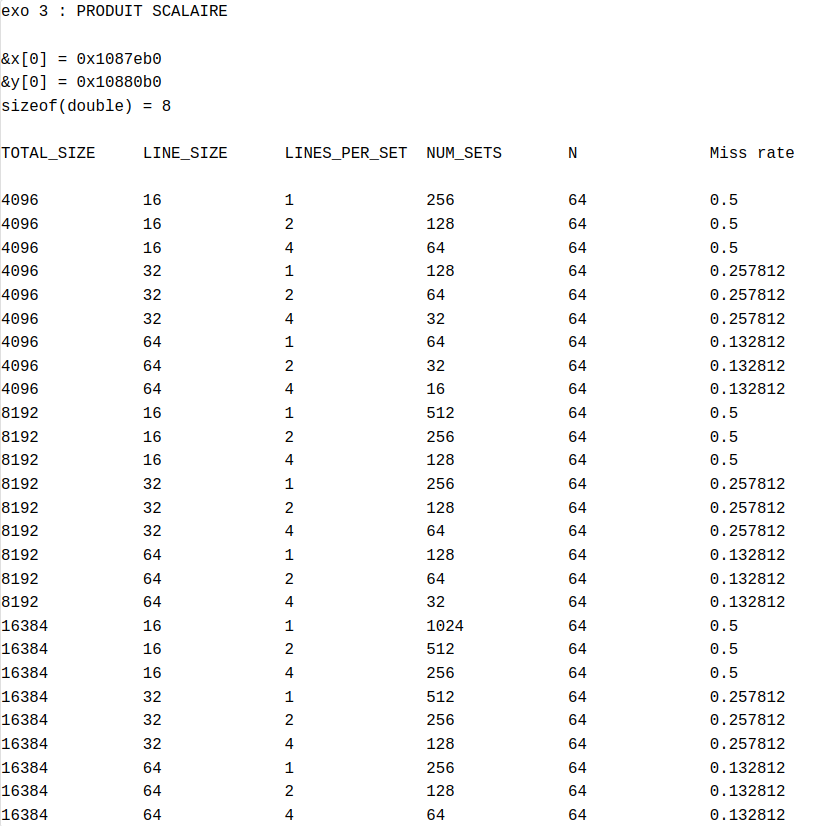
\includegraphics[width=0.75\linewidth]{1_scal_64.png}
    \caption{$\text{N}=64$}
    \label{fig:1_64}
\end{subfigure}
\begin{subfigure}[H]{0.5\linewidth}
    \centering
    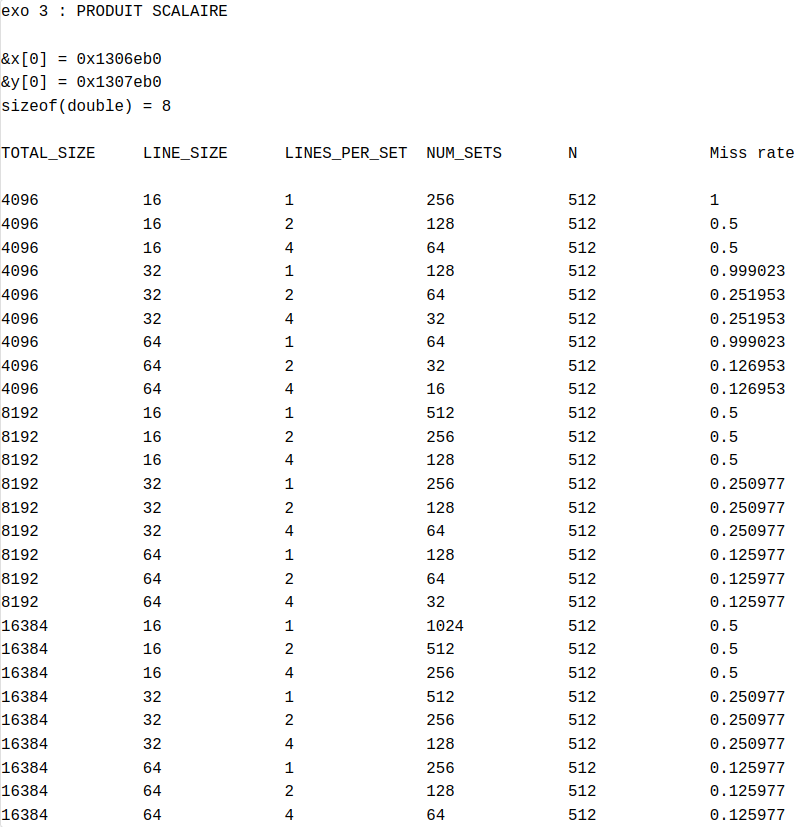
\includegraphics[width=0.75\linewidth]{1_scal_512.png}
    \caption{$\text{N}=512$}
    \label{fig:1_512}
\end{subfigure}\par\bigskip
\begin{subfigure}[H]{0.5\linewidth}
    \centering
    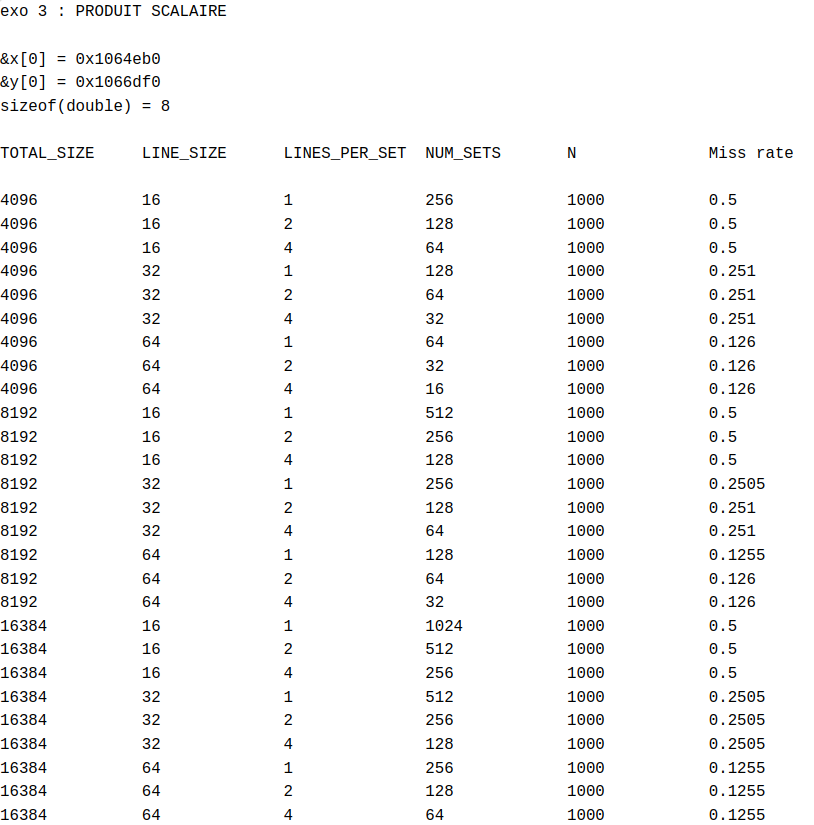
\includegraphics[width=0.75\linewidth]{1_scal_1000.png}
    \caption{$\text{N}=1000$}
    \label{fig:1_1000}
\end{subfigure}
\begin{subfigure}[H]{0.5\linewidth}
    \centering
    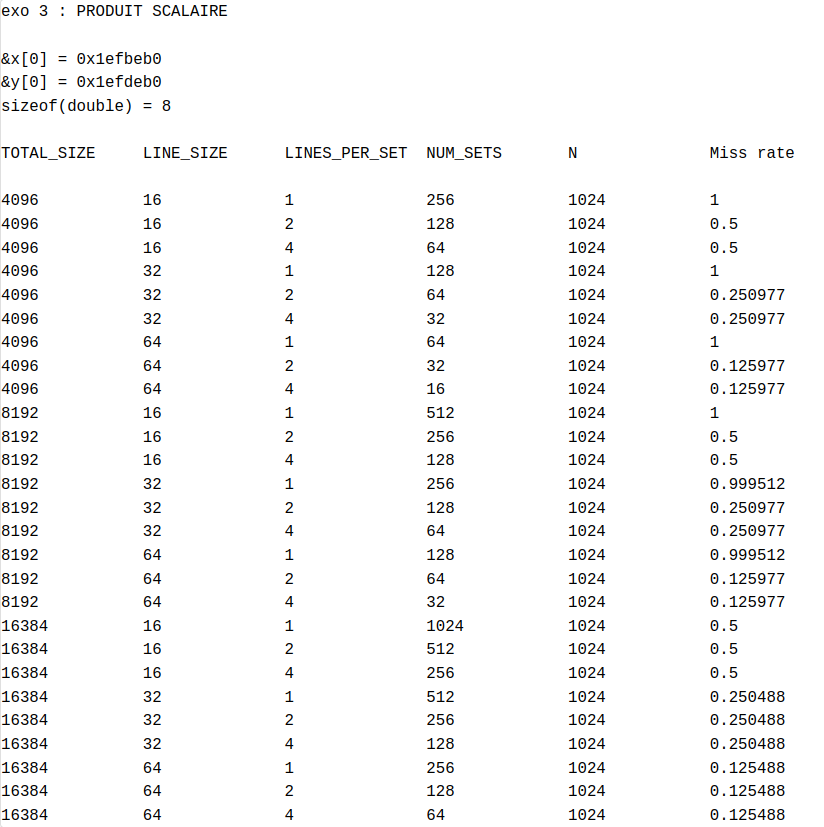
\includegraphics[width=0.75\linewidth]{1_scal_1024.png}
    \caption{$\text{N}=1024$}
    \label{fig:1_1024}
\end{subfigure}
\begin{subfigure}[H]{0.5\linewidth}
    \centering
    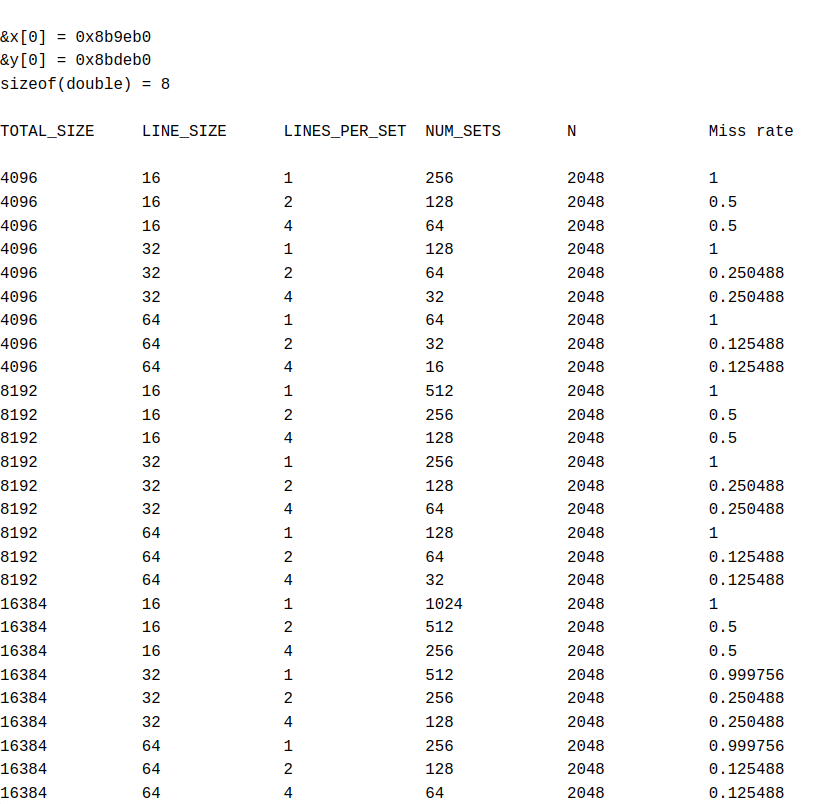
\includegraphics[width=0.75\linewidth]{1_scal_2048.png}
    \caption{$\text{N}=2048$}
    \label{fig:1_2048}
\end{subfigure}
\end{figure}


\newpage
\section{Produit matriciel - vecteur}



\begin{figure}[H]
\begin{subfigure}[H]{0.5\linewidth}
    \centering
    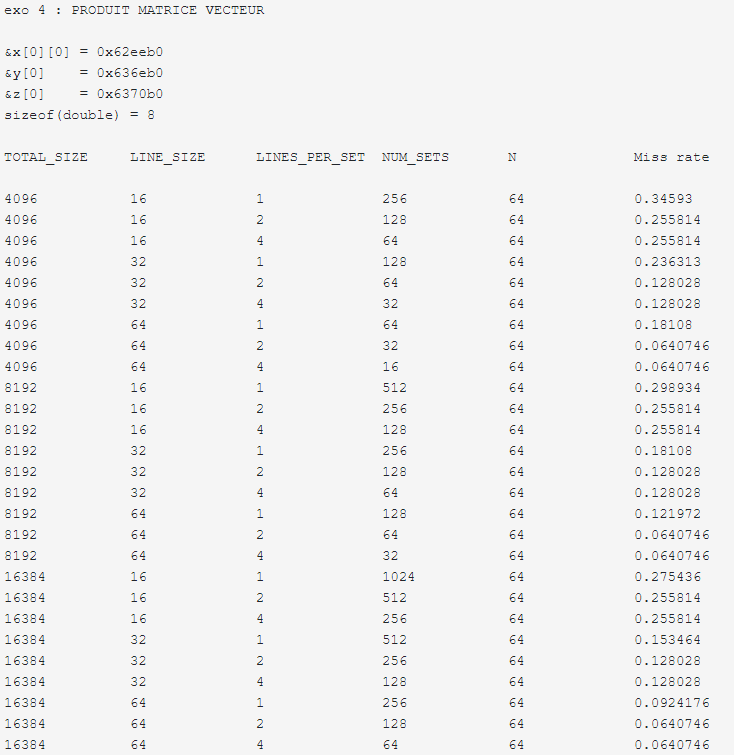
\includegraphics[width=0.75\linewidth]{2_vect_64.png}
    \caption{$\text{N}=64$}
    \label{fig:2_64}
\end{subfigure}
\begin{subfigure}[H]{0.5\linewidth}
    \centering
    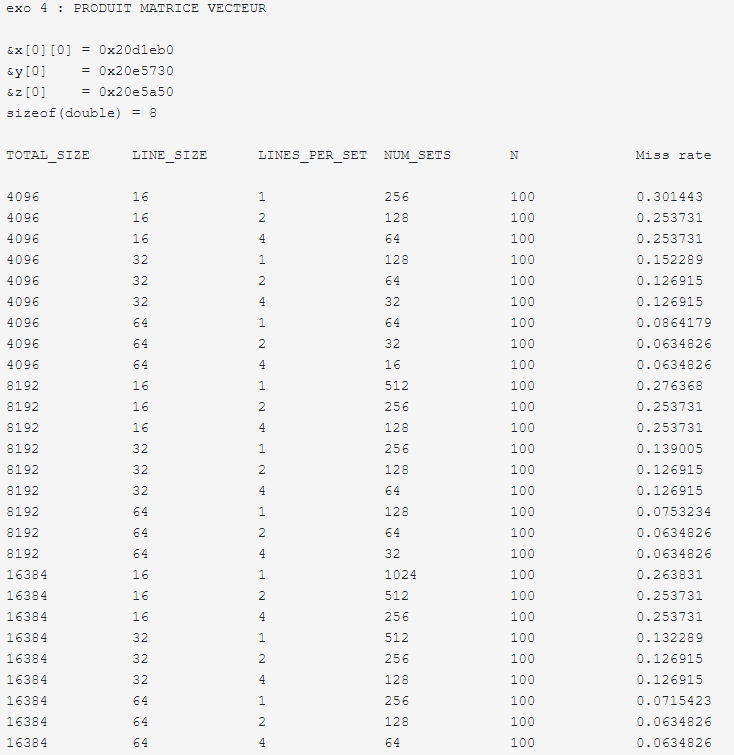
\includegraphics[width=0.75\linewidth]{2_vect_100.png}
    \caption{$\text{N}=100$}
    \label{fig:2_100}
\end{subfigure}\par\bigskip
\begin{subfigure}[H]{0.5\linewidth}
    \centering
    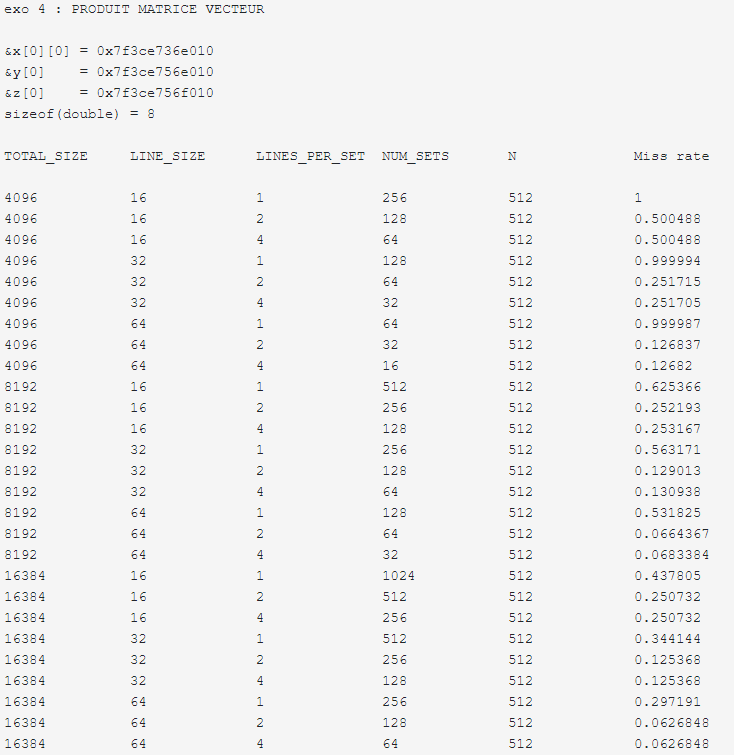
\includegraphics[width=0.75\linewidth]{2_vect_512.png}
    \caption{$\text{N}=512$}
    \label{fig:2_512}
\end{subfigure}
\begin{subfigure}[H]{0.5\linewidth}
    \centering
    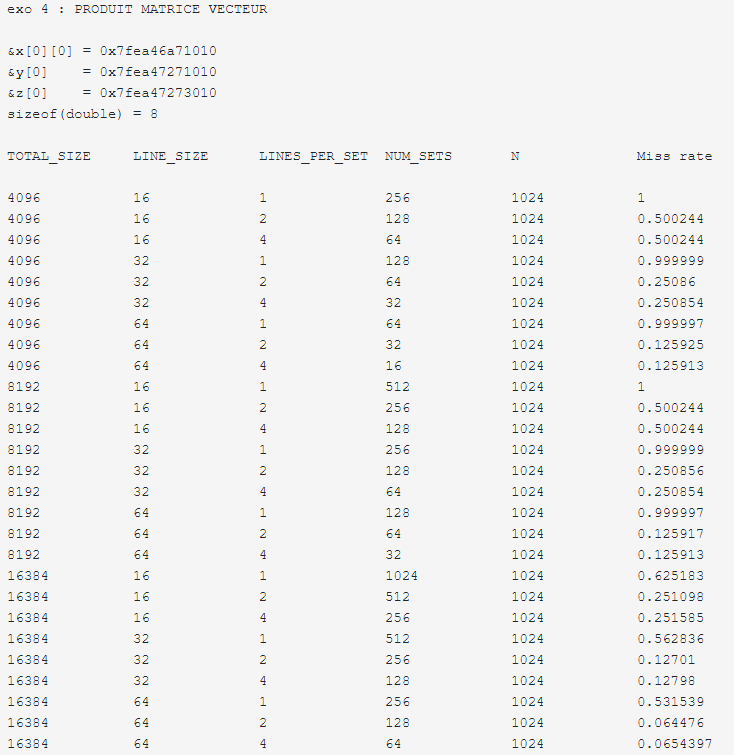
\includegraphics[width=0.75\linewidth]{2_vect_1024.png}
    \caption{$\text{N}=1024$}
    \label{fig:2_1024}
\end{subfigure}
\end{figure}

\newpage
\section{Produit matriciel ijk}

\begin{figure}[H]
\begin{subfigure}[H]{0.5\linewidth}
    \centering
    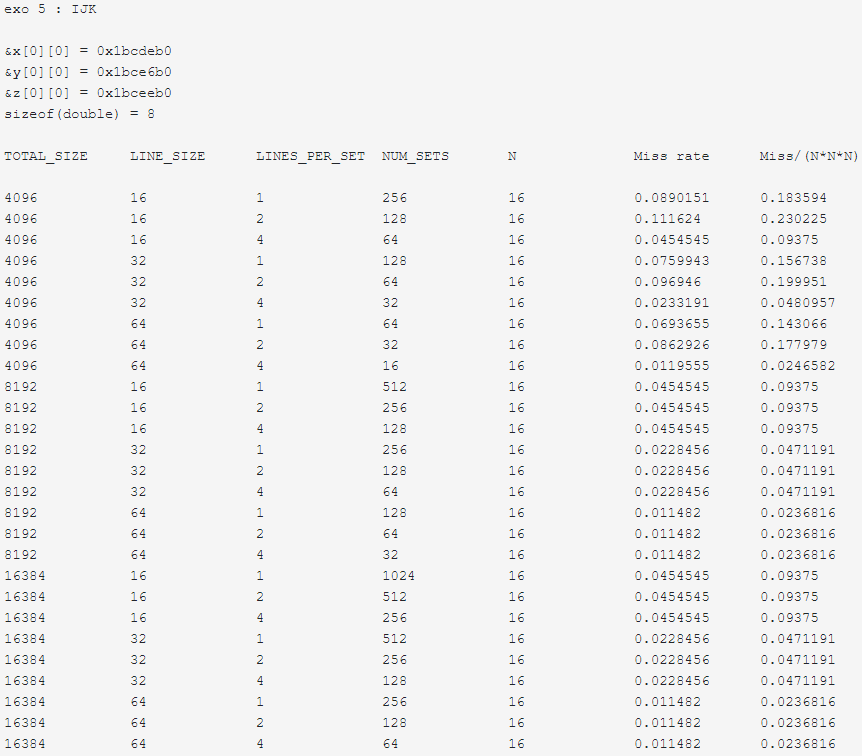
\includegraphics[width=0.75\linewidth]{3_ijk_16.png}
    \caption{$\text{N}=16$}
    \label{fig:3_16}
\end{subfigure}
\begin{subfigure}[H]{0.5\linewidth}
    \centering
    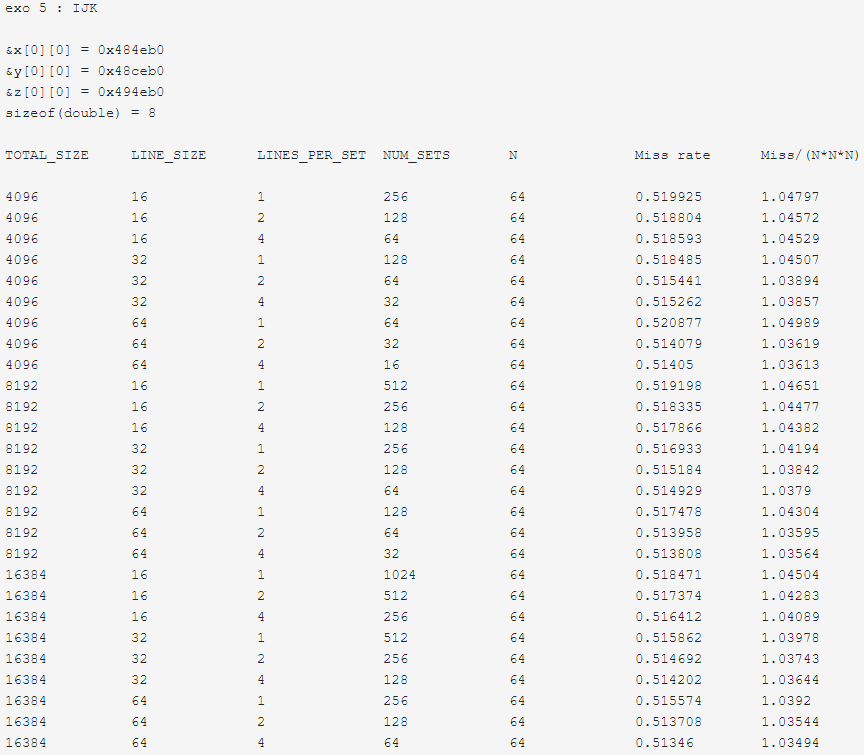
\includegraphics[width=0.75\linewidth]{3_ijk_64.png}
    \caption{$\text{N}=64$}
    \label{fig:3_64}
\end{subfigure}\par\bigskip
\begin{subfigure}[H]{0.5\linewidth}
    \centering
    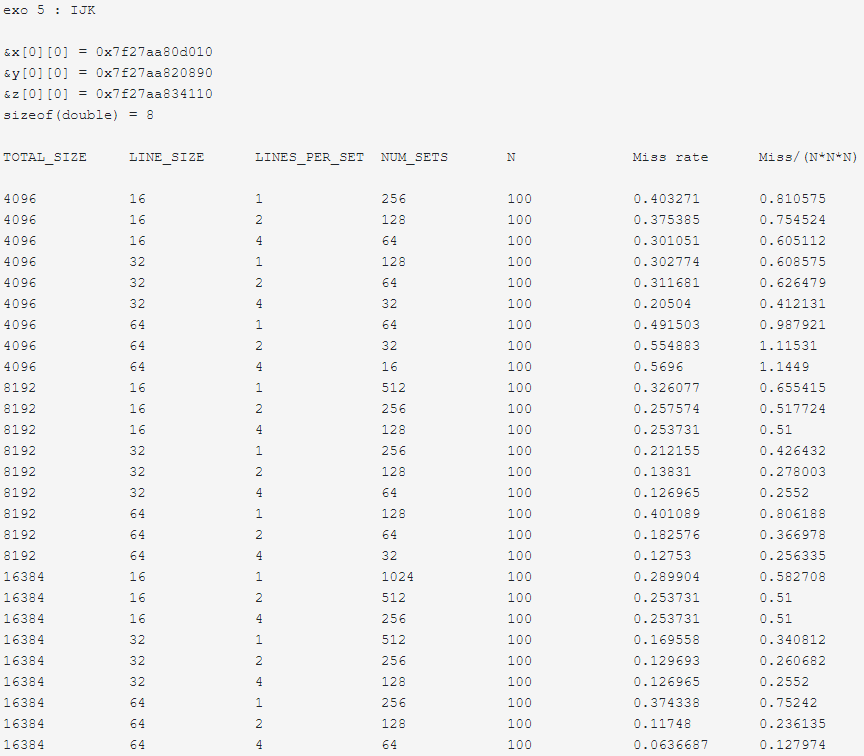
\includegraphics[width=0.75\linewidth]{3_ijk_100.png}
    \caption{$\text{N}=100$}
    \label{fig:3_100}
\end{subfigure}
\end{figure}

\newpage
\section{Produit matriciel ijk après transposition}

\begin{figure}[H]
\begin{subfigure}[H]{0.5\linewidth}
    \centering
    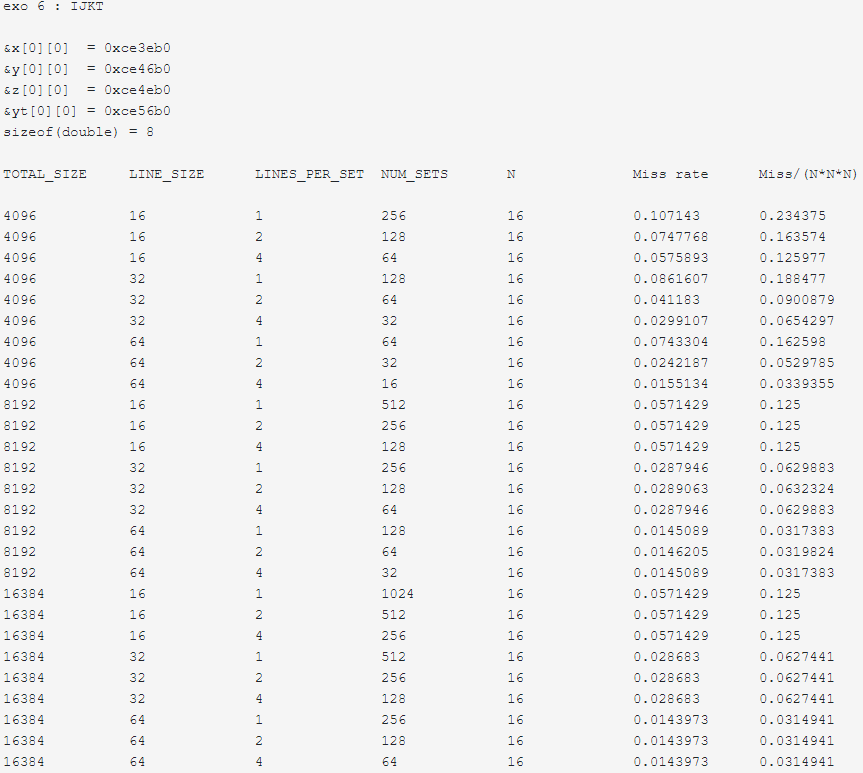
\includegraphics[width=0.75\linewidth]{4_ijkt_16.png}
    \caption{$\text{N}=16$}
    \label{fig:4_16}
\end{subfigure}
\begin{subfigure}[H]{0.5\linewidth}
    \centering
    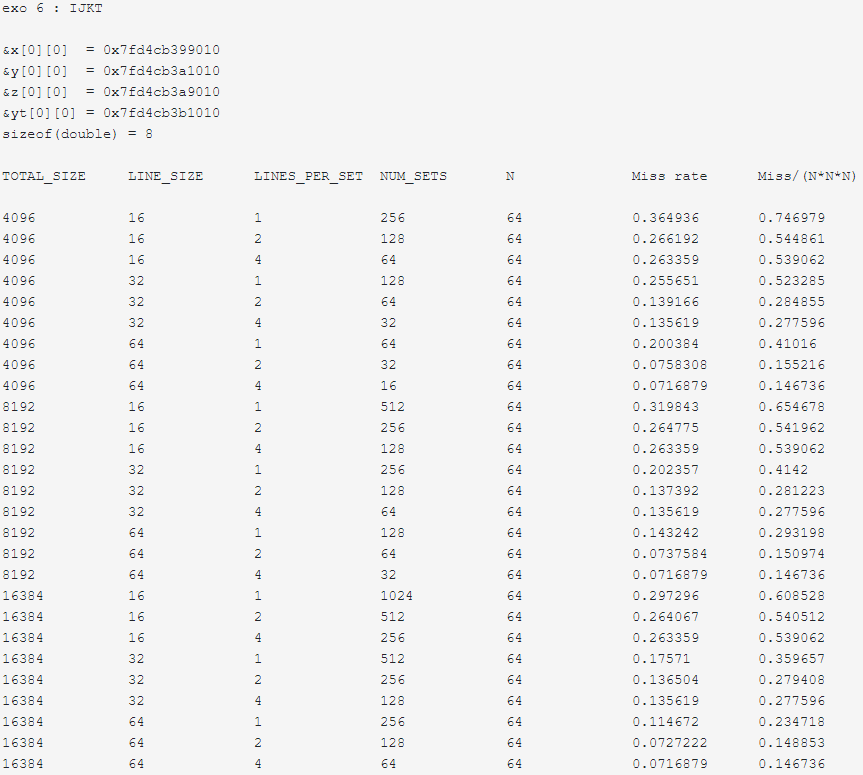
\includegraphics[width=0.75\linewidth]{4_ijkt_64.png}
    \caption{$\text{N}=64$}
    \label{fig:4_64}
\end{subfigure}\par\bigskip
\begin{subfigure}[H]{0.5\linewidth}
    \centering
    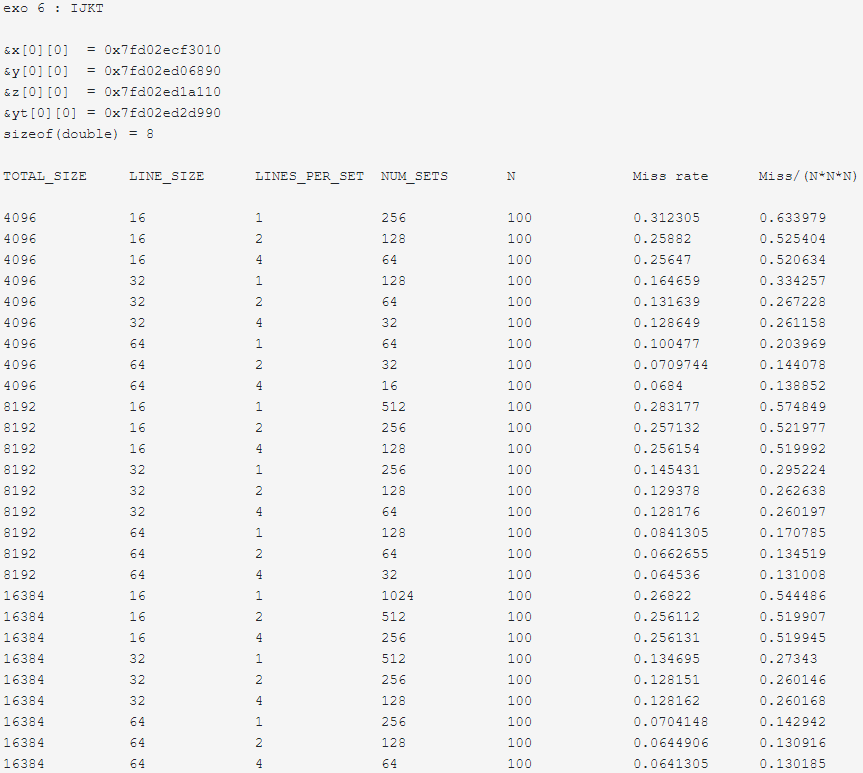
\includegraphics[width=0.75\linewidth]{4_ijkt_100.png}
    \caption{$\text{N}=100$}
    \label{fig:4_100}
\end{subfigure}
\end{figure}

\end{document}
